\section{Linux Networking}
\label{sec:linuxNetworking}

Esta sección recopilará todos los conceptos y herramientas relacionadas con la parte de Networking en Linux, que son fundamentales para el desarrollo, análisis y validación de este proyecto.


%%%%%%%%%%%%%%%%%%%%%%%%%%%%%%%%%%%%%%%%%%%%%%%%%%%%%%%%%%%%%%%%%%%%%%%%%%%%%%%%%%%%%%%%%%

\subsection{Interfaz virtual - \texttt{tun/tap}}
\label{linuxNetworking_tuntap}

En el mundo de las redes siempre se habla de las interfaces tun/tap de forma indistinta cuando van a utilizarse, sin embargo, cada una tiene su cometido. Como se ha indicado, en networking, las interfaces TUN/TAP son interfaces virtuales que se crean y se gestionan en espacio de kernel. Mencionar que como estas interfaces son virtuales y se gestionan directamente vía softaware, no como las interfaces reales que se gestionan con unos drivers diferentes, cada interfaz con su driver específico de la interfaz.  Los drivers de las interfaces TUN/TAP se crearon en los 2000 como una unión de los avances de los drivers desarrollados en las comunidades de Solaris, Linux, BSD. Actualmente los drivers solo tienen mantenimiento por los kernels de linux y FreeBSD. Ambos tipos de interfaces se utilizan para tunelado, pero no pueden ser utilizadas a la vez dado que trabajan en niveles distintos. Las TUN, de \textit{network \textbf{TUN}nel}, emula la capa de red y puede llegar hacer reenvío de los paquetes. En cambio las interfaces TAP,  trabajan en capa 2 solo en capa dos, y emulan un equipo que trabaja en dicha capa, como por ejemplo un switch \cite{tuntap1}. Por tanto, hay que dejar claro lo que se puede llegar a realizar con cada interfaz (Ver figura \ref{fig:linux1}).

\begin{itemize}
    \item \texttt{TUN} se puede llegar a utilizar para routing.
    \item \texttt{TAP} se puede llegara utilizar para crear un bridge.
\end{itemize}

Generalmente, cuando los paquetes son enviados por el sistema operativo a través de una interfaz TUN/TAP,  serán recibidos por algún programa de espacio de usuario, el cual, está enganchado directamente en la interfaz. Cualquier programa de espacio de usuario podrá pasar paquetes por las interfaces, y las interfaces virtuales se lo pasarán al \textit{stack} de red por defecto, emulando la recepción de los paquetes inyectados desde espacio de usuario.\\
\\
% fig
\begin{figure}[ht]
    \centering
    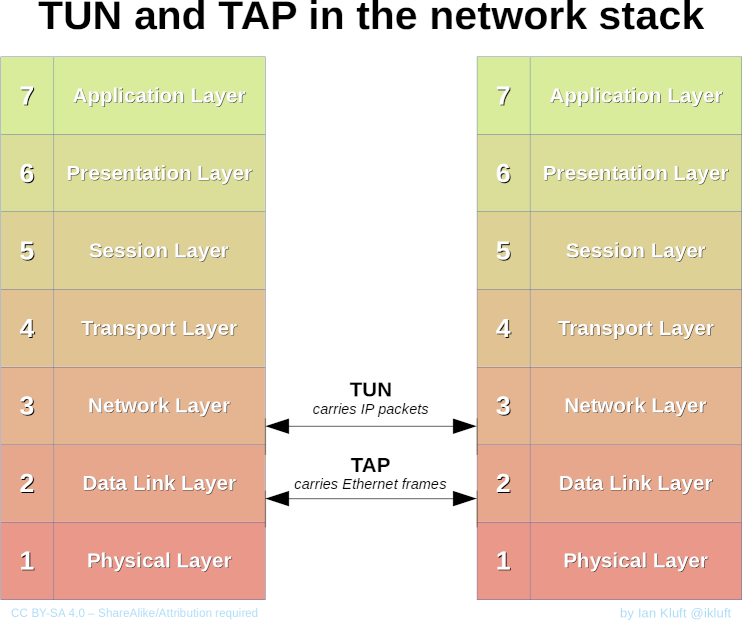
\includegraphics[width=\textwidth]{archivos/img/teoria/linux1.png}
    \caption{Diagrama de funcionamiento de las interfaces virtuales TUN/TAP \cite{tuntap2}}
    \label{fig:linux1}
\end{figure}

Para la creación de estas interfaces lo podemos hacer por ioctl o podemos hacerlo más fácil a través del binario tunctl o en su defecto con el comando de \texttt{tuntap} del set de herramientas iproute2. A continuación, en el bloque \ref{code:tun_tap_use} se indican todos los comandos necesarios para trabajar con las interfaces TUN/TAP.\\

\begin{lstlisting}[language= bash, style=Consola, caption={Manejo de interfaces TUN - TAP},label=code:tun_tap_use]
    # En caso de querer utilizar tunctl hay que instalar el binario
    sudo apt install -y uml-utilities
    
    # Para crear una un interfaz podemos hacer lo siguiente
    tunctl -t {nombre_tun}

    # Para eliminarla
    tunctl -d {nombre_tun}

    # Para crear interfaces de tipo TAP hay que hacer lo siguiente
    tunctl -p -t {nombre_tun}
    
    # El comando análogo con iproute2 sería el siguiente
    ip tuntap add dev {nombre_tun} mode {tun|tap}
\end{lstlisting}
\vspace{0.5cm}

En caso de que queramos comprobar que las interfaces se han creado correctamente siempre se puede hacer uso de la herramienta \texttt{ethtool}. A continuación, en la figura \ref{fig:linux2}, se puede ver como en el campo \texttt{bus-info} nos indica que tipo de interfaz es.

% fig
\begin{figure}[ht]
    \centering
    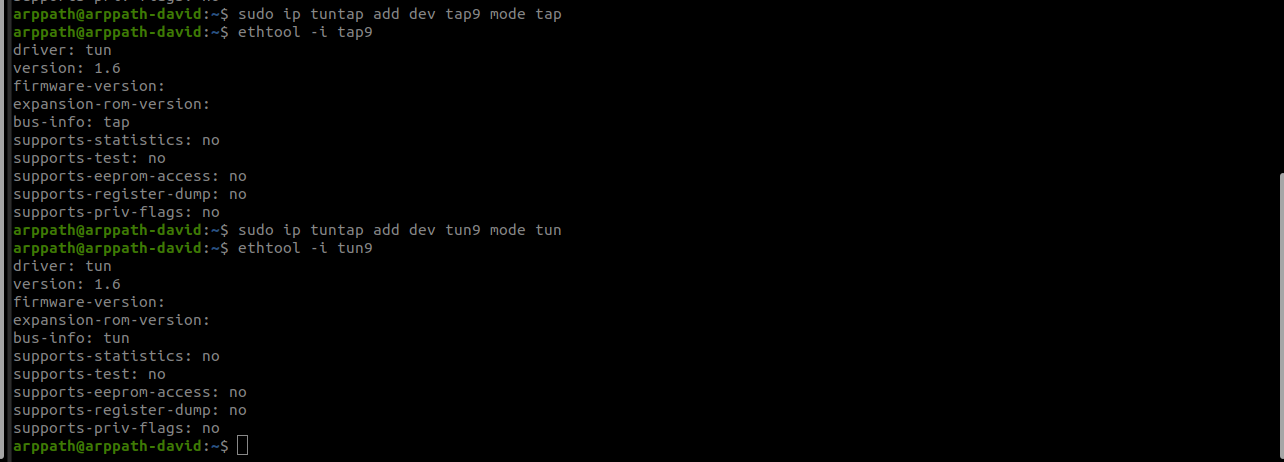
\includegraphics[width=\textwidth]{archivos/img/teoria/linux2.png}
    \caption{Comprobación con \texttt{ethtool} de tipo de interfaz virtual.}
    \label{fig:linux2}
\end{figure}


%%%%%%%%%%%%%%%%%%%%%%%%%%%%%%%%%%%%%%%%%%%%%%%%%%%%%%%%%%%%%%%%%%%%%%%%%%%%%%%%%%%%%%%%%%
\subsection{Interfaz virtual - \texttt{veth}}
\label{linuxVeths}
Las \gls{veth} son interfaces de Ethernet virtuales creadas como un par de interfaces interconectadas entre sí. El modelo funcional es sencillo: los paquetes enviados desde una interfaz son recibidos por la otra de forma directa, similar al funcionamiento de las \textit{pipes} (mecanismo de comunicación interprocesos en linux). Una característica interesante de estas interfaces es que su gestión está asociada, lo que significa que si se habilita una extremo de la \gls{veth}, el otro extremo también se habilitará, y si se deshabilita o se elimina un extremo de un par de \gls{veth}, el otro extremo también se verá afectado \cite{veth}.\\
\\
Es muy común utilizar las \gls{veth} para interconectar \textit{Network Namespaces}. Al saber que estas interfaces estarán conectadas de forma directa, se puede utilizar este enlace como una pasarela entre dos \textit{Network Namespaces}. De esta manera, se pueden interconectar dos \textit{stacks} independientes de red. Más adelante se verá que alguno de los emuladores más utilizados para comprobar despliegues de red \gls{sdn} hace uso de estas interfaces. Y podemos ir más allá, no sé quiere tampoco entrar en el mundo de los contenedores dado que el proyecto no va a utilizarlos, pero simplemente indicar que estas interfaces también son utilizadas para la interconexión y contenedores de Docker \cite{veths1}. La creación y eliminación de este tipo de interfaces se puede observar en el bloque de código \ref{code:iproute2_veth}. Se recuerda que se necesitan permisos de root para realizar estas operaciones.

\begin{lstlisting}[language= bash, style=Consola, caption={Uso de las interfaces Veths},label=code:iproute2_veth]
    # COn este comando se crean un par interfaces veth
    ip link add {veth1_name} type veth peer name {veth2_name}
    
    # Solo hace falta indicar uno de los dos nombres del par de Veths
    ip link delete {veth_name}
    
\end{lstlisting}
\vspace{0.5cm}


%%%%%%%%%%%%%%%%%%%%%%%%%%%%%%%%%%%%%%%%%%%%%%%%%%%%%%%%%%%%%%%%%%%%%%%%%%%%%%%%%%%%%%%%%%

\subsection{Herramienta \texttt{TC}}


En Linux, \gls{tc} es un subsistema del kernel, que tiene una interfaz en espacio de usuario que se utiliza para controlar y gestionar el tráfico de red. Proporciona una serie de herramientas y mecanismos para aplicar políticas de \gls{qos}, limitar el ancho de banda, establecer prioridades de tráfico, realizar filtrado y dar forma al tráfico de red \cite{tc1}. Se ha añadido esta sección a la memoria dado que la mayoría de emuladores de red en Linux suelen hacer uso de esta herramienta para modelar los enlaces de las topologías emuladas. El \gls{tc}  se utiliza principalmente para las siguientes tareas.

\begin{itemize}
    \item Control de ancho de banda: Nos permite limitar la cantidad de ancho de banda que un flujo de datos específico puede utilizar. Esto es útil para evitar que un flujo de tráfico acapare todo el ancho de banda y afecte el rendimiento de otros flujos.

    \item Priorización de tráfico: Permite asignar prioridades diferentes a los diferentes flujos de datos. Esto asegura que ciertos flujos de tráfico, como VoIP o similares al ser más sensibles, tengan prioridad sobre otros, como la descarga de archivos donde la latencia y el jitter no son un problema, pero si la integridad.

    \item Modelado y conformación de tráfico: Permite dar forma al tráfico de red mediante la definición de límites en el ritmo de transmisión. Esto es útil para evitar congestiones en la red y garantizar un flujo de tráfico constante y uniforme.

    \item Marcado y filtrado de paquetes: Permite clasificar y filtrar paquetes de acuerdo a diferentes criterios, como direcciones IP, puertos, protocolos, etc. Esto permite aplicar políticas específicas a ciertos flujos de datos o bloquear ciertos tipos de tráfico no deseado. Esta funcionalidad es útil, pero está duplicada con otros submódulos del kernel de Linux, como por ejemplo las \texttt{ip-tables}.
\end{itemize}

El procesamiento del tráfico para conseguir llevar a cabo las tareas anteriormente mencionadas, se emplean tres tipos de objetos: \textbf{qdiscs}, \textbf{classes} y \textbf{filters} \cite{tc1}.

\subsubsection{Qdiscs}

El objeto qdics, que significa ``Quality-Deficit Inverse Congestion Control Scheduler" (Planificador de Control de Congestión Inverso de Calidad-Deficit), es un concepto fundamental en el networking de Linux que determina el orden en el que los miembros de la cola, en este caso los paquetes, son seleccionados para su servicio. \\
\\
Por ejemplo, cuando una herramienta de espacio de usuario necesita transmitir un paquete en un momento dado, ese paquete se entrega al \textit{stack} de red y, finalmente, llega a la interfaz de red por la cual será transmitido. En ese momento, el paquete se encuentra encolado en una cola, esperando ser transmitido. Estas colas son gestionadas por un qdics. El qdics por defecto en Linux es un pfifo, que significa ``Priority-First-In, First-Out", señalar el concepto de prioridad, dado que es fundamental. Por tanto lo podemos ver como una cola pura en la que se sigue el orden de llegada (\textit{first-in}) y se atienden los paquetes en ese orden siempre y cuando no haya alguna directriz de prioridad, con una limitación en el tamaño de la cola en términos del número de paquetes que puede contener.

\subsubsection{Classes}


Las clases pueden entenderse como sub-qdics dentro de un qdics. Una clase puede contener a su vez otras clases, formando sistemas de  \gls{qos} detallados, como se muestra en la figura \ref{fig:linuxNet_tc}. Cuando los paquetes son recibidos en una cola gestionada por un qdics, pueden ser encolados en base a las características del paquete en otras colas administradas por otras clases. Esto permite, por ejemplo, priorizar el envío de datos de una aplicación sobre otra. Para lograrlo, los paquetes de ambas aplicaciones se clasificarán en clases diferentes, asignándole a una clase más prioridad que a la otra. Esto implica asignar más recursos de transmisión y recepción a la clase prioritaria.\\
\\
En resumen, las clases en el contexto de los qdics representan subdivisiones que permiten una gestión más detallada del tráfico de red. Al agrupar paquetes en diferentes clases y asignar prioridades, se puede establecer un control más minucioso sobre la transmisión y recepción de datos, lo que facilita la implementación de políticas de \gls{qos} y la asignación de recursos de manera más eficiente.
% fig
\begin{figure}[ht]
    \centering
    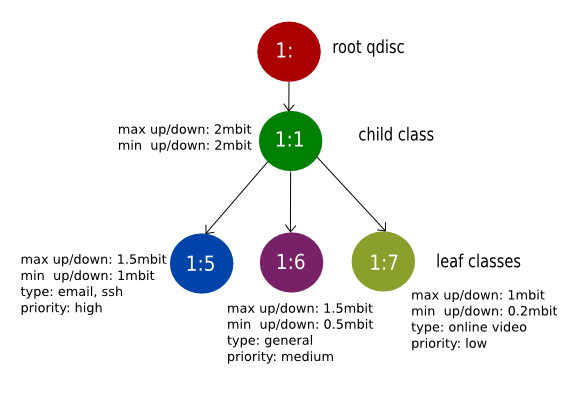
\includegraphics[width=0.7\textwidth]{archivos/img/teoria/tc_qdisc_example_implementation.png}
    \caption{Mecanimo de calidad de servicio implementado con clases y sub-clases \cite{qdiscs}}
    \label{fig:linuxNet_tc}
\end{figure}


\subsubsection{Filters}

En el contexto de \gls{tc} en Linux, los filtros son objetos utilizados para seleccionar y clasificar paquetes de red con el fin de aplicar acciones específicas sobre ellos. Los filtros permiten establecer reglas que determinan cómo se deben tratar los paquetes en función de diferentes criterios, como direcciones IP, puertos, protocolos, etiquetas VLAN, campos de encabezado, entre otros. Los filtros en \gls{tc} se utilizan en conjunción con los qdics para controlar y gestionar el tráfico de red de manera más granular. Se pueden aplicar diferentes acciones a los paquetes que coinciden con los criterios definidos por los filtros, como encolarlos en clases específicas, modificar sus encabezados, descartarlos, redirigirlos a interfaces de red diferentes, entre otras opciones. Existen varios tipos de filtros disponibles en \gls{tc}, entre ellos podemos ver los siguientes.

\begin{itemize}
    \item Tipo U32: Permite filtrar paquetes basados en campos de encabezado, como direcciones IP, puertos y protocolos.
    \item Tipo Basic: Permite filtrar paquetes utilizando criterios básicos como direcciones IP de origen y destino, puertos y protocolos.
    \item Tipo Route: Permite filtrar paquetes en función de las rutas de red.
    \item Tipo \gls{bpf}: Permite utilizar programas \gls{bpf} para filtrar y procesar paquetes.
\end{itemize}

Estos son solo algunos ejemplos de los tipos de filtros disponibles en \gls{tc}. Cada tipo de filtro tiene su propia sintaxis y opciones de configuración específicas. Por tanto, los filtros en \gls{tc} se utilizan para seleccionar y clasificar paquetes de red en función de diferentes criterios. Estos filtros permiten aplicar acciones específicas a los paquetes que coinciden con los criterios definidos, lo que facilita la gestión y el control del tráfico de red en Linux.


%%%%%%%%%%%%%%%%%%%%%%%%%%%%%%%%%%%%%%%%%%%%%%%%%%%%%%%%%%%%%%%%%%%%%%%%%%%%%%%%%%%%%%%%%%

\subsection{Namespaces}
\label{namespaces}

Una \textit{Namespace} se utiliza para encapsular un recurso del sistema operativo en una abstracción que engaña a los procesos dentro de esa \textit{Namespace} haciéndoles creer que tienen su propia instancia aislada del recurso en cuestión, separada del sistema real. Los cambios realizados en los recursos aislados solo son visibles para los procesos que pertenecen a esa \textit{Namespace}, mientras que son invisibles para otros procesos que pertenecen al sistema o a otra \textit{Namespace}.\\
\\
Existen varios tipos de \textit{Namespaces}, los cuales se detallan en la tabla \ref{tab:linux_ns}. Cada tipo de \textit{Namespace} tiene diversos usos y aplicaciones, pero uno de los más relevantes es el de los contenedores. Los contenedores proporcionan un entorno aislado para ejecutar aplicaciones o herramientas. Actualmente, los contenedores más populares son los de Docker, una plataforma ampliamente utilizada en el mundo del desarrollo de software. Docker aprovecha las bondades del kernel de Linux para aislar recursos y crear instancias aisladas del sistema Host sobre el cual se ejecutan. Utiliza la API proporcionada por el kernel para crear y destruir \textit{Namespaces} según sea necesario. En esencia, Docker es un conjunto de llamadas al sistema que se encarga de gestionar \textit{Namespaces}. Además de la gestión de \textit{Namespaces}, Docker proporciona otras características útiles, como el mecanismo de \textit{copy-on-write} y una configuración de red en modo \textit{bridge} hacia el exterior. Sin embargo, en su núcleo, Docker es simplemente un\textit{wrapper} que facilita la gestión de \textit{Namespaces} con el objetivo de implementar contenedores.

% \begin{table}[ht]
%     \centering
%     \resizebox{\textwidth}{!}{%
%         \begin{tabular}{|l|l|}
%             \hline
%             \rowcolor[HTML]{EFEFEF}
%             \multicolumn{1}{|c|}{\cellcolor[HTML]{EFEFEF}{\color[HTML]{24292E} \textbf{Tipo de Namespace}}} & \multicolumn{1}{c|}{\cellcolor[HTML]{EFEFEF}{\color[HTML]{24292E} \textbf{Descripción}}}                                                                                                                                                     \\ \hline
%             \textbf{Cgroup}                                                                                 & \begin{tabular}[c]{@{}l@{}}Namespace utilizada generalmente para establecer unos limites de recursos,  por ejemplo, \\ CPU, memoria, lecturas y escrituras a disco, de todos los procesos que corran dentro de dicha Namespace.\end{tabular} \\ \hline
%             Time                                                                                            & Namespace para establecer una hora del sistema diferente a la del sistema.                                                                                                                                                                   \\ \hline
%             \textbf{Network}                                                                                & Namespace utilizada para tener una replica aislada del stack de red del sistema, dentro del propio sistema.                                                                                                                                  \\ \hline
%             \textbf{User}                                                                                   & Namespace utilizada para tener aislados a un grupo de usuarios.                                                                                                                                                                              \\ \hline
%             \textbf{PID}                                                                                    & Namespace utilizada para tener identificadores de proceso independientes de otras namespaces.                                                                                                                                                \\ \hline
%             \textbf{IPC}                                                                                    & Namespace utilizada para aislar los mecanismos de comunicación entre procesos.                                                                                                                                                               \\ \hline
%             \textbf{Uts}                                                                                    & Namespace utilizada para establecer un nombre de Host y nombre de dominio diferentes de los establecidos en el sistema                                                                                                                       \\ \hline
%             \textbf{Mount}                                                                                  & Namespace utilizada para aislar los puntos de montaje en el sistema de archivos.                                                                                                                                                             \\ \hline
%         \end{tabular}%
%     }
%     \caption{Resumen de los tipos de Namespaces en el Kernel de Linux}
%     \label{tab:linux_ns}
% \end{table}


\begin{table}[ht]
    \centering
    \resizebox{\textwidth}{!}{%
        \begin{tabular}{|l|l|}
            \hline
            \rowcolor[HTML]{EFEFEF}
            \multicolumn{1}{|c|}{\cellcolor[HTML]{EFEFEF}{\color[HTML]{24292E} \textbf{Tipo de Namespace}}} & \multicolumn{1}{c|}{\cellcolor[HTML]{EFEFEF}{\color[HTML]{24292E} \textbf{Descripción}}}                                                                                                                                   \\ \hline
            \textbf{Cgroup}                                                                                 & \begin{tabular}[c]{@{}l@{}}Namespace utilizado generalmente para establecer límites de recursos,\\ como CPU, memoria, lecturas y escrituras a disco, para todos los procesos\\ dentro de la misma Namespace. \end{tabular} \\ \hline
            Time                                                                                            & \begin{tabular}[c]{@{}l@{}}Namespace utilizado para establecer una hora del sistema diferente\\ a la del sistema global.\end{tabular}                                                                                      \\ \hline
            \textbf{Network}                                                                                & \begin{tabular}[c]{@{}l@{}}Namespace utilizado para crear una réplica aislada del stack de red \\ del sistema dentro del propio sistema.      \end{tabular}                                                                \\ \hline
            \textbf{User}                                                                                   & Namespace utilizado para aislar un grupo de usuarios.                                                                                                                                                                      \\ \hline
            \textbf{PID}                                                                                    & \begin{tabular}[c]{@{}l@{}}Namespace utilizado para tener identificadores de proceso independientes\\ de otras namespaces. \end{tabular}                                                                                   \\ \hline
            \textbf{IPC}                                                                                    & Namespace utilizado para aislar los mecanismos de comunicación entre procesos.                                                                                                                                             \\ \hline
            \textbf{Uts}                                                                                    & \begin{tabular}[c]{@{}l@{}}Namespace utilizado para establecer un nombre de host y nombre de dominio \\ diferentes de los establecidos en el sistema.      \end{tabular}                                                   \\ \hline
            \textbf{Mount}                                                                                  & Namespace utilizado para aislar los puntos de montaje en el sistema de archivos.                                                                                                                                           \\ \hline
        \end{tabular}%
    }
    \caption{Resumen de los tipos de Namespaces en el Kernel de Linux}
    \label{tab:linux_ns}
\end{table}


\subsubsection{Persistencia de las Namespaces}


Según la página man-page sobre las \textit{Namespaces} \cite{ns}, es importante tener en cuenta que las \textit{Namespaces} tienen una vida finita. La duración de una \textit{Namespace} dependerá de si está siendo referenciada, lo que significa que vivirá mientras siga siendo referenciada y será destruida cuando deje de serlo. Comprender este concepto de vida finita es crucial para tener una mejor comprensión del funcionamiento interno de Mininet o Mininet-WiFi, ya que estas herramientas aprovechan estos conceptos para optimizar las operaciones y mejorar el rendimiento de sus respectivos emuladores.\\
\\
Actualmente, una \textit{Namespace} puede ser referenciada de tres maneras diferentes:

\begin{itemize}
    \item Siempre que haya un proceso en ejecución dentro de dicha \textit{Namespace}.
    \item Siempre que haya abierto un descriptor de archivo para el archivo identificador de la \textit{Namespace} (por ejemplo, \texttt{/proc/{pid}/ns/{tipo\_namespace}}).
    \item Siempre que exista un \textit{bind-mount} del archivo (\texttt{/proc/{pid}/ns/{tipo\_namespace}}) de la \textit{Namespace} en cuestión.
\end{itemize}

Si ninguna de estas condiciones se cumple, el kernel eliminará automáticamente la \textit{Namespace}. En el caso de una \textit{Network Namespace}, las interfaces que se encuentren dentro de la \textit{Namespace} que está siendo eliminada volverán a la \textit{Network Namespace} predeterminada \cite{ns}. Es fundamental tener en cuenta estos detalles, ya que ayudan a comprender cómo se manejan las \textit{Namespaces} y cómo se gestionan los recursos en el contexto de Mininet o Mininet-WiFi.

\subsubsection{Concepto de las Network Namespaces}

Una vez comprendido el concepto de \textit{Namespace} en Linux, es necesario introducir las \textit{Network Namespace}, las cuales desempeñarán un papel fundamental en las plataformas utilizadas para emular. Estas \textit{Network Namespace} consisten en réplicas lógicas del \textit{stack} de red predeterminado de Linux, que incluye rutas, tablas ARP, Iptables e interfaces de red \cite{netns}.\\
\\
Linux se inicia con una \textit{Network Namespace} predeterminada, conocida como el espacio \textit{root}, que tiene su propia tabla de rutas, tabla ARP, Iptables e interfaces de red. Sin embargo, también es posible crear \textit{Network Namespace} adicionales que no son predeterminadas, crear nuevos dispositivos dentro de esos espacios de nombres o trasladar dispositivos existentes de un espacio de nombres a otro. La herramienta más sencilla para llevar a cabo todas estas tareas de gestión con las Netns es \texttt{iproute2} (consulte el Anexo \ref{iproute2}). Esta herramienta, utilizando el módulo \texttt{netns}, permite gestionar todo lo relacionado con las \textit{Network Namespace} con nombre (\textit{named network namespaces}). \\
\\
La característica ``con nombre" significa que todas las \textit{Network Namespace} administradas mediante \texttt{iproute2} serán persistentes, ya que se realizará un \textit{bind-mount} del archivo identificador de la \textit{Namespace} en cuestión con su nombre correspondiente en el directorio \texttt{/var/run/netns}. A continuación, en el bloque \ref{code:iproute2_ns}, se enumeran los comandos más comunes utilizados para gestionar las \textit{Network Namespace}. Se asume que estos comandos se ejecutan con privilegios de root.\\

\begin{lstlisting}[language= bash, style=Consola, caption={Casos de uso de las Netns},label=code:iproute2_ns]
    # Con el siguiente comando creamos una network namespace
    ip netns add {netns_name}
    
    # Listamos las Named Network Namespaces :)
    ip netns list
    
    # Movemos una interfaz a una Network Namespace determinada
     ip netns set {netns_name} Veth
    
    # Ejecutamos un comando dentro de una Network Namespace
    ip netns exec {netns_name} {cmd}
    
    # De esta forma, eliminamos una Network Namespace
    ip netns del {netns_name}
    
\end{lstlisting}
\vspace{0.2cm}

\subsubsection{Comunicación inter-Namespaces: \glsentryshort{veth}}
\label{linuxVeths}

Por lo tanto, se puede representar el siguiente diagrama básico para ilustrar el funcionamiento de un par de interfaces \gls{veth} asignadas a diferentes \textit{Network Namespaces}. Como se muestra en la Figura \ref{fig:linuxNet_veth}, ambas interfaces están directamente conectadas internamente en el Kernel. Si se generan paquetes desde una \textit{Network Namespace} hacia la otra, estos paquetes viajarán desde un extremo de la \gls{veth} directamente al otro extremo de la \gls{veth} a través del Kernel, sin ser percibidos por la \textit{Network Namespace} predeterminada. Esta configuración resulta muy útil para establecer enlaces entre nodos de red independientes. Los nodos se replicarán utilizando \textit{Network Namespaces} y los enlaces se establecerán utilizando pares de interfaces \gls{veth}. Estos mecanismos son ampliamente utilizados por herramientas de emulación de redes como Mininet o Mininet-WiFi, lo cual se explicará en detalle más adelante.

\begin{figure}[ht]
    \centering
    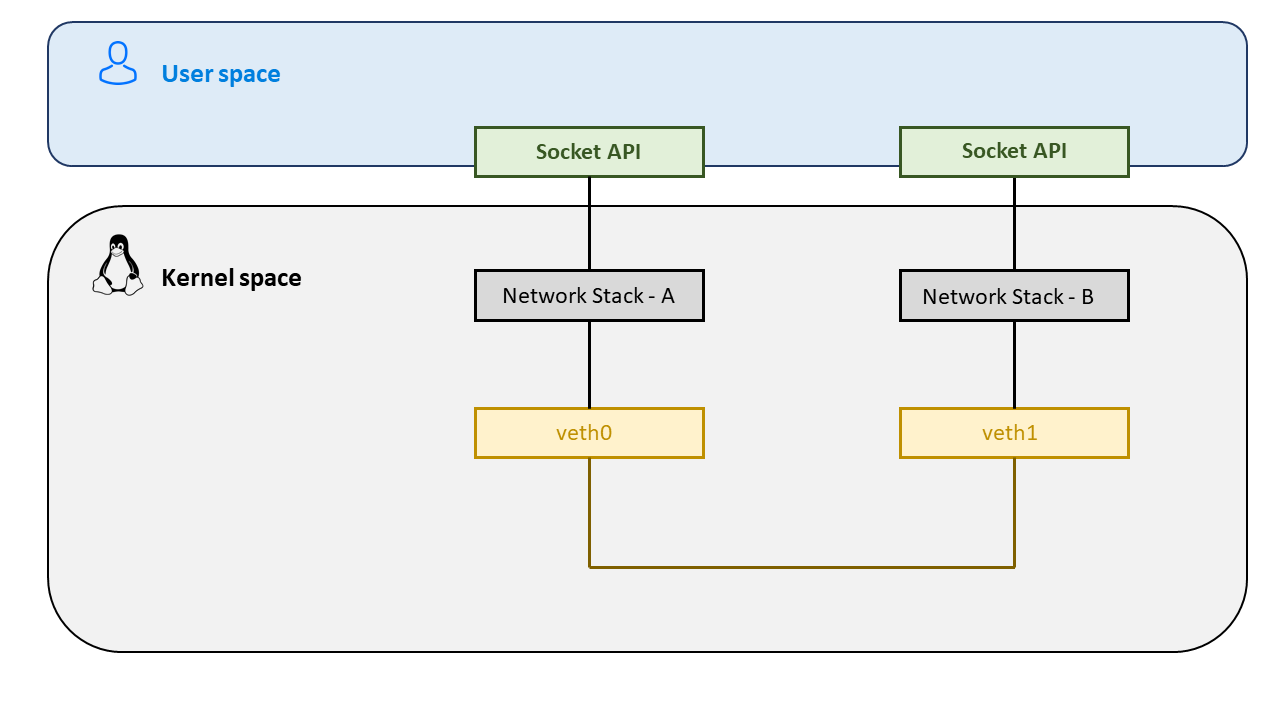
\includegraphics[width=0.9\textwidth]{archivos/img/teoria/user_kernel.png}
    \caption{Enlace entre interfaces Veth separadas en dos Network Namespaces \cite{carrascal2020diseno}}
    \label{fig:linuxNet_veth}
\end{figure}


%%%%%%%%%%%%%%%%%%%%%%%%%%%%%%%%%%%%%%%%%%%%%%%%%%%%%%%%%%%%%%%%%%%%%%%%%%%%%%%%%%%%%%%%%%

\subsection{Linux Wireless Subsystem}
\label{linux_w}

El subsistema inalámbrico de Linux consiste en un conjunto de módulos presentes en el kernel de Linux. Estos módulos se encargan de manejar la configuración del hardware según el estándar \texttt{ieee80211}, así como de la gestión de la transmisión y recepción de paquetes de datos. En la arquitectura de este subsistema, el primer bloque que encontramos al analizar de abajo hacia arriba es el módulo mac80211\_hwsim. Este módulo es responsable de crear las interfaces inalámbricas virtuales en Mininet-WiFi.\\
\\
El objetivo principal del módulo mac80211\_hwsim es facilitar a los desarrolladores de controladores de tarjetas inalámbricas la prueba de su código y la interacción con el siguiente bloque llamado mac80211. Las interfaces virtualizadas no tienen ciertas limitaciones presentes en el hardware real, lo que facilita la realización de diversas pruebas con diferentes configuraciones sin estar limitados por recursos materiales. Este módulo generalmente recibe un parámetro único, que es el número de ``radios" o interfaces virtuales que se desean virtualizar. Dado que las posibilidades ofrecidas por este módulo eran algo limitadas, se han creado varios wrappers que proporcionan funcionalidades adicionales más allá de las que ofrece el módulo en sí. La mayoría de las herramientas creadas hacen uso de la biblioteca Netlink para comunicarse directamente con el subsistema en el kernel y lograr configuraciones adicionales, como agregar un RSSI en particular, o asignar un nombre a la interfaz. Un ejemplo de dicha herramienta es \texttt{mac80211\_hwsim\_mgmt}, que es utilizada por Mininet-WiFi para gestionar la creación de interfaces inalámbricas en cada nodo que las requiere.\\
\\
Es importante destacar el cambio de paradigma que existe en el subsistema inalámbrico de Linux en relación al concepto de interfaz. Generalmente, se piensa en una interfaz como un elemento que gestiona el acceso al medio en la capa dos y el propio hardware en la capa física, como sería el caso de una interfaz Ethernet. Sin embargo, en el subsistema inalámbrico se descompone la interfaz en dos capas \cite{8330098}. Una de ellas es la capa física (\textit{PHY}), donde se puede gestionar, por ejemplo, en qué canal está operando la tarjeta inalámbrica emulada. La otra capa es el acceso al medio, representado por las interfaces virtuales que se derivan de una tarjeta inalámbrica. La idea detrás de este paradigma es que se pueden tener \textit{N} interfaces virtuales asociadas a una misma tarjeta inalámbrica, aunque es importante destacar que estas interfaces virtuales funcionan principalmente como interfaces Ethernet (a excepción de las que están en modo monitor).

\subsubsection{Limitaciones del módulo \texttt{mac80211\_hwsim}}
\label{limits}

Como se mencionó anteriormente, la mayoría de las interfaces virtuales asociadas a una tarjeta inalámbrica emulada son del tipo Ethernet, lo que implica que todos los paquetes que se reciben están encapsulados con cabeceras Ethernet. Esta situación plantea una limitación, ya que en ciertos casos de uso se desea manipular las cabeceras WiFi. Sin embargo, debido a que las interfaces virtuales son principalmente del tipo Ethernet, no es posible lograr este objetivo.

% foto downstream
% figura escenario
\begin{figure}[ht]
    \centering
    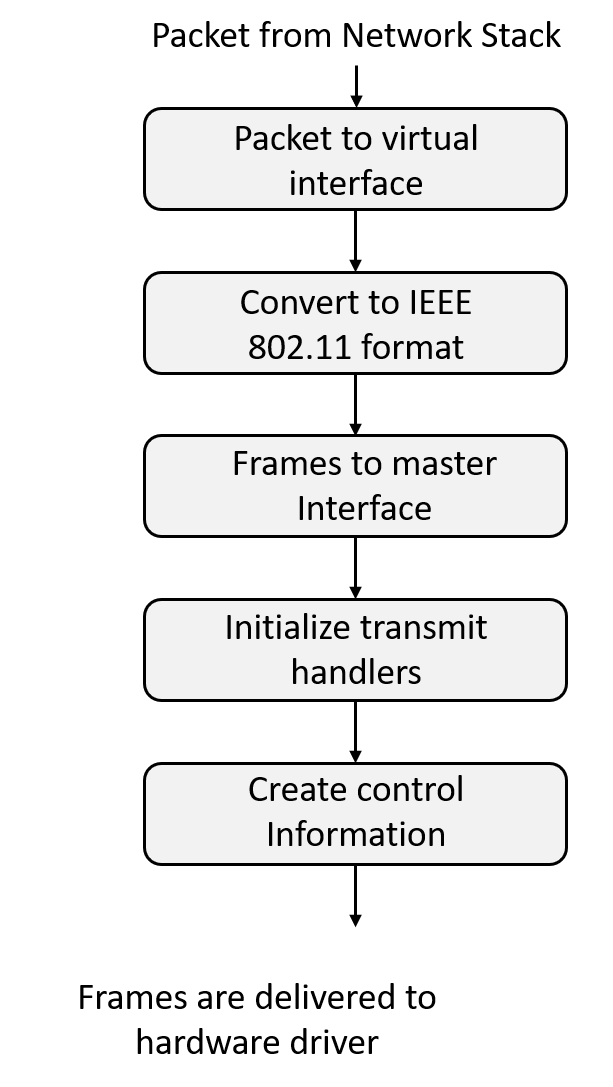
\includegraphics[width=0.3\textwidth]{archivos/img/dev/p4-wifi/analysis/linux_wireless_subsystem_tx.png}
    \caption{Pipeline de transmisión del módulo mac80211\_hwsim \cite{5415877}}
    \label{fig:analysis_p4_wifi_7}
\end{figure}

Sin embargo, ¿cuál es el motivo de convertir las cabeceras WiFi a cabeceras Ethernet? Hasta ahora, la única razón que se ha encontrado para esta decisión de diseño es simplificar la implementación de los controladores que funcionan con el módulo mac80211\_hwsim. Estos controladores convierten las cabeceras a Ethernet y las entregan al stack de red para que las gestione como paquetes de una red cableada convencional. Este enfoque permite que las aplicaciones que operan a nivel de interfaz sean más fácilmente compatibles y extrapolables.

% foto upstream
% figura escenario
\begin{figure}[ht]
    \centering
    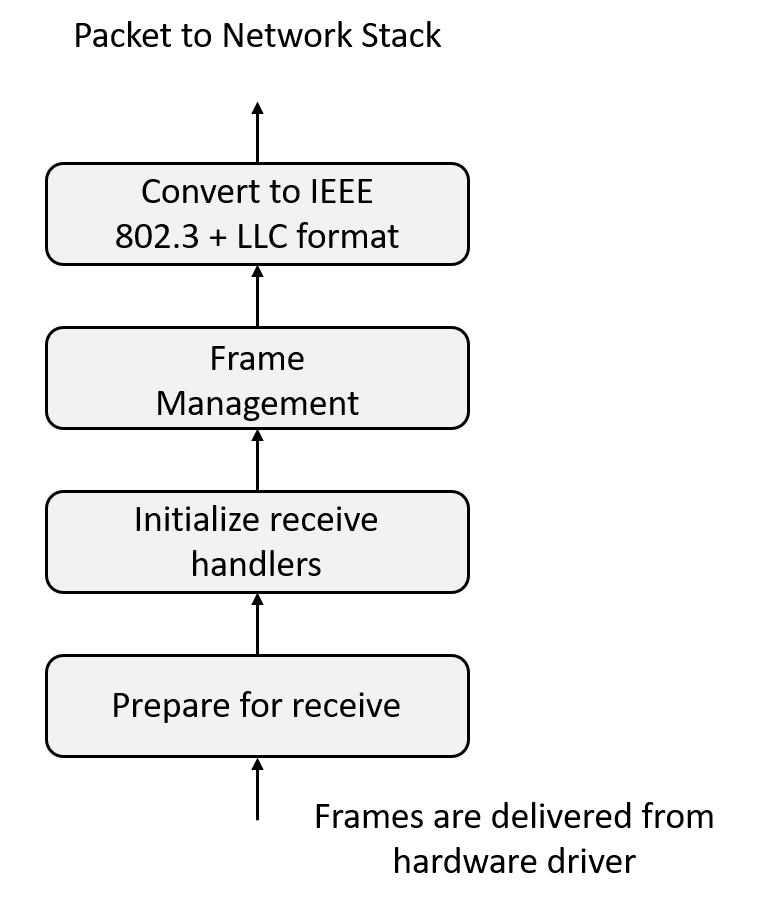
\includegraphics[width=0.4\textwidth]{archivos/img/dev/p4-wifi/analysis/linux_wireless_subsystem_rx.png}
    \caption{Pipeline de recepción del módulo mac80211\_hwsim \cite{5415877}}
    \label{fig:analysis_p4_wifi_8}
\end{figure}

Es importante mencionar que esto implica un consumo considerable de recursos, ya que el paquete se encola hasta tres veces (controlador, cola Ethernet, cola de la disciplina de planificación de colas) y se requiere tiempo y recursos para llevar a cabo la traducción de las cabeceras. Puedes encontrar la función en el kernel donde se realiza este proceso \href{https://elixir.bootlin.com/linux/latest/C/ident/__ieee80211_data_to_8023}{aquí}\footnote{\url{https://elixir.bootlin.com/linux/latest/C/ident/__ieee80211_data_to_8023}}. Esta situación ocurre generalmente, pero no siempre, ya que el único modo en el que una interfaz puede recibir paquetes WiFi es en el modo monitor. Sin embargo, el modo monitor está diseñado únicamente para la escucha de paquetes, no para la transmisión. Este modo se puede llevar al límite al realizar una inyección de paquetes (packet injection) a través de la interfaz. Por tanto, cuando se trabaje con este módulo del kernel, se tiene que ser cosciente que los paquetes que se verán por las tarjetas WiFi emuladas serán paquetes con cabeceras 802.3 en vez de 802.11.